\chapter{SYSTEM DESIGN AND ANALYSIS}
\section{System Analysis}
"Mitho Delivery" project involves breaking the project into small parts and creating prototypes to get feedback from users quickly. Rapid Application Development (RAD) is a fast approach to building software applications. RAD saves time by reusing existing components and focuses on user involvement. It's a flexible method that adapts to changes and helps identify and fix problems early.\\
Rapid Application Development (RAD) consists of four main phases that guide the development process:

\begin{enumerate}

\item \textbf{Requirements Planning:} In this phase, the project team identifies and understands the application's goals and user requirements.
\item \textbf{Prototyping:} The prototyping phase focuses on creating a working model or prototype of the application. 
\item \textbf{Iterative Development:} The iterative development phase involves building the application in multiple stages or iterations. Each iteration typically focuses on a specific set of features or functionalities. 
\item \textbf{Deployment and Feedback:} Once the application is developed, it is deployed for real-world use. This phase involves the final implementation and integration of the application into the production environment. Feedback from end-users and stakeholders is collected to identify any areas that need further refinement or improvement.
\end{enumerate}

\section{Requirement Analysis}
\subsubsection{Functional Requirements}

    
Functional requirements for Mitho Delivery, an online food delivery system: 	
\begin{enumerate} 
\item User Registration and Login: Users can create an account and securely log in to the platform. 
\item Menu Browsing: Users can browse menus, view dish price and descriptions.
\item Order Placement: Users can select items from the menu, customize orders, and add them to the cart for checkout. 
\item Cart Management: Users can review and modify items in their cart before finalizing the order. 
\item Customer Support: Users have access to customer support channels for assistance, issue reporting, and inquiries.
\end{enumerate}
\subsubsection{Non Functional Requirements}
Non-functional requirements for Mitho Delivery, an online webpage for food delivery system, may include:
\begin{enumerate}
    \item Usability: Ensure a user-friendly interface and easy navigation for all users.
    \item Performance: Provide fast loading times and efficient handling of multiple user interactions.
    \item Reliability: Maintain high availability and minimize downtime.
    \item Scalability: Accommodate future growth and handle increased user demand without performance issues.
    \item Compatibility: Support various devices, browsers, and operating systems for broad accessibility.
    \item Accessibility: Comply with accessibility standards to enable users with disabilities to access and use the platform effectively.
\end{enumerate}

\newpage
\subsection{Feasibility Analysis}
\subsection*{Economically Feasibility}
Utilizing free and open-source cross-platform software development tools like HTML, CSS,
JavaScript, and PHP offers significant economic feasibility advantages. These tools eliminate
the need for expensive proprietary software licenses, provide access to extensive community
support, and enable platform independence, resulting in cost savings. Their flexibility and
customization options allow tailored solutions without vendor lock-in. Furthermore, the scalability
and collaborative nature of open-source tools facilitate future enhancements and tap into a vast
pool of talent. Hence, it makes our system economically feasible.

\subsection*{Operational Feasibility}
Operational feasibility for a food delivery system involves the assessment of its practical viability. This encompasses the verification of adequate resources such as delivery staff and vehicles and the compatibility of the system with prevailing technology and processes. Adherence to legal regulations and the positive reception of customers are also encompassed. Through the consideration of these factors, the potential for the successful implementation of the food delivery system can be ascertained.

\subsection*{Technical Feasibility}
The technical feasibility of the Mitho Delivery food delivery system involves assessing its potential for construction utilizing available technology. The imperative is to ensure the smooth operational performance and the safeguarding of user data. Through consideration of these factors, the determination of the successful construction and operation of the Mitho Delivery webpage can be reached.

\newpage
\subsection{Data Modelling(ER-Diagram)}
An entity relationship diagram (ERD), also known as an entity relationship model, is a graphical representation that depicts relationships among people, objects, places, concepts or events within an information technology (IT) system.

\begin{figure}[h]    
    \rotatebox{90}{
        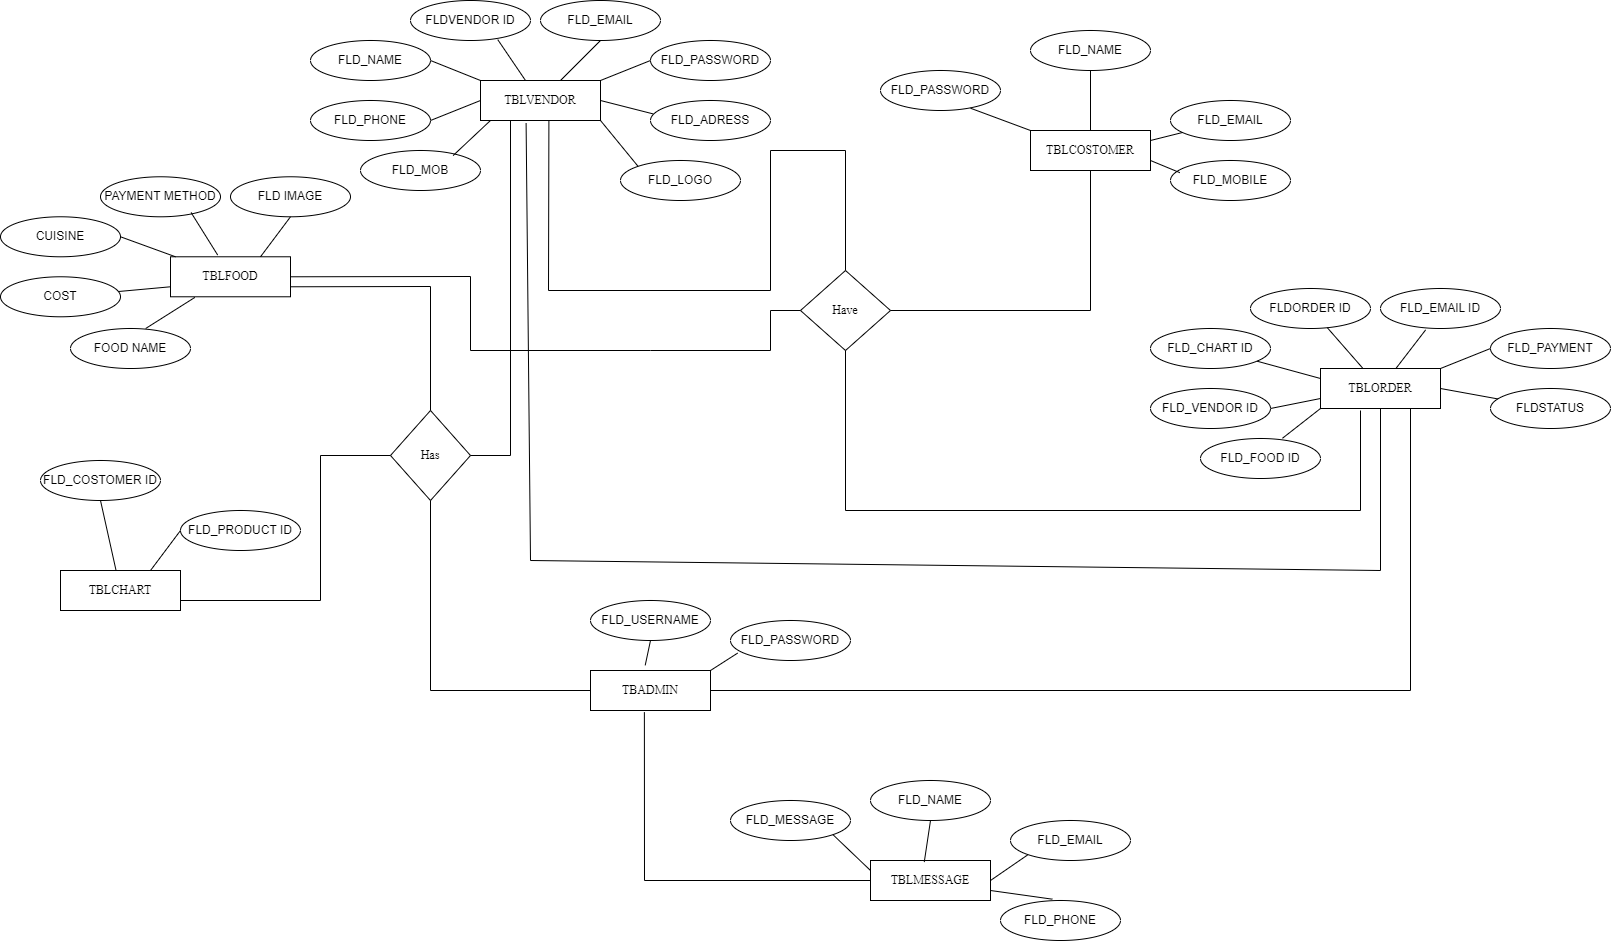
\includegraphics[scale=0.3]{img/Graphics/ER DIAGRAM PROJECT.png}}
    \caption{ER Diagram}
\end{figure}


\newpage
\subsection{Physical DFD}
\begin{figure}[h]
    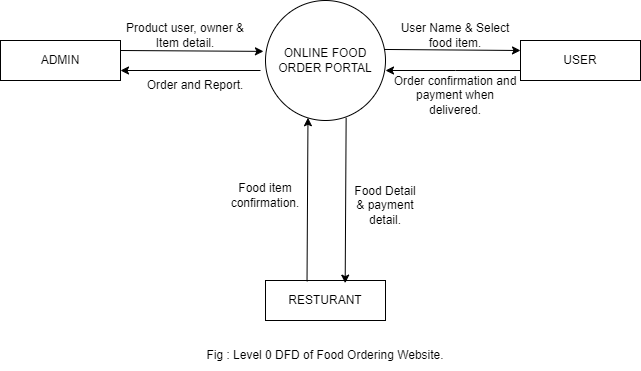
\includegraphics[scale=0.6]{img/Graphics/Level DFD.png}
    \caption{Physical DFD level}
\end{figure}

\newpage

\section{System Design}
\subsection{Use Case Diagram}
\begin{figure}[h]
    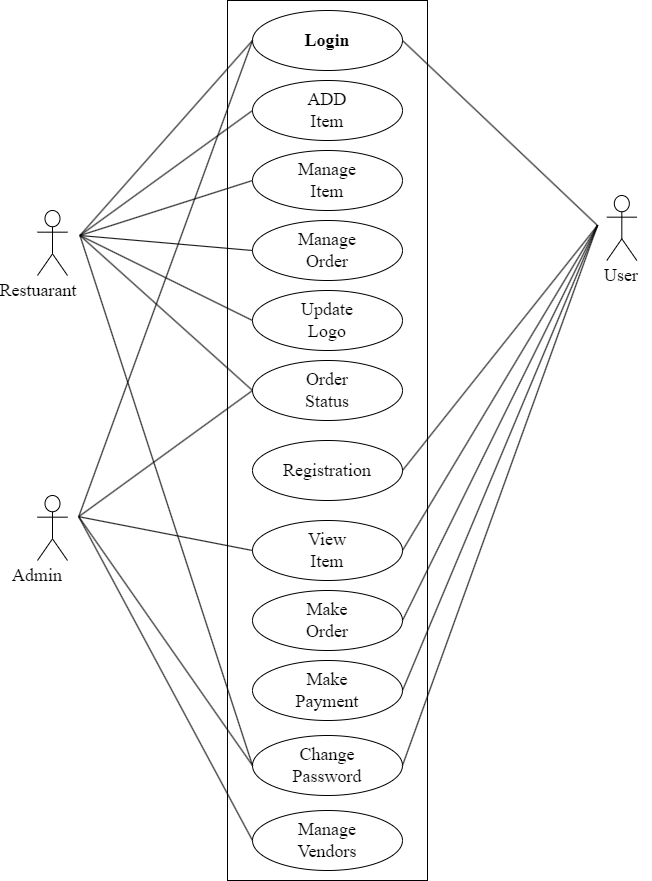
\includegraphics[scale=0.5]{img/Graphics/useCase.drawio.png}
    \caption{Use Case Diagram}
\end{figure}

\newpage
\subsection{Interface Design}
User interface (UI) design is the process designers use to build interfaces in software or computerized devices, focusing on looks or style. Designers aim to create interfaces which users find easy to use and pleasurable. UI design refers to graphical user interfaces and other forms—\\\\
Below is the login page ui of our project.
\begin{figure}[h]
    \centering
    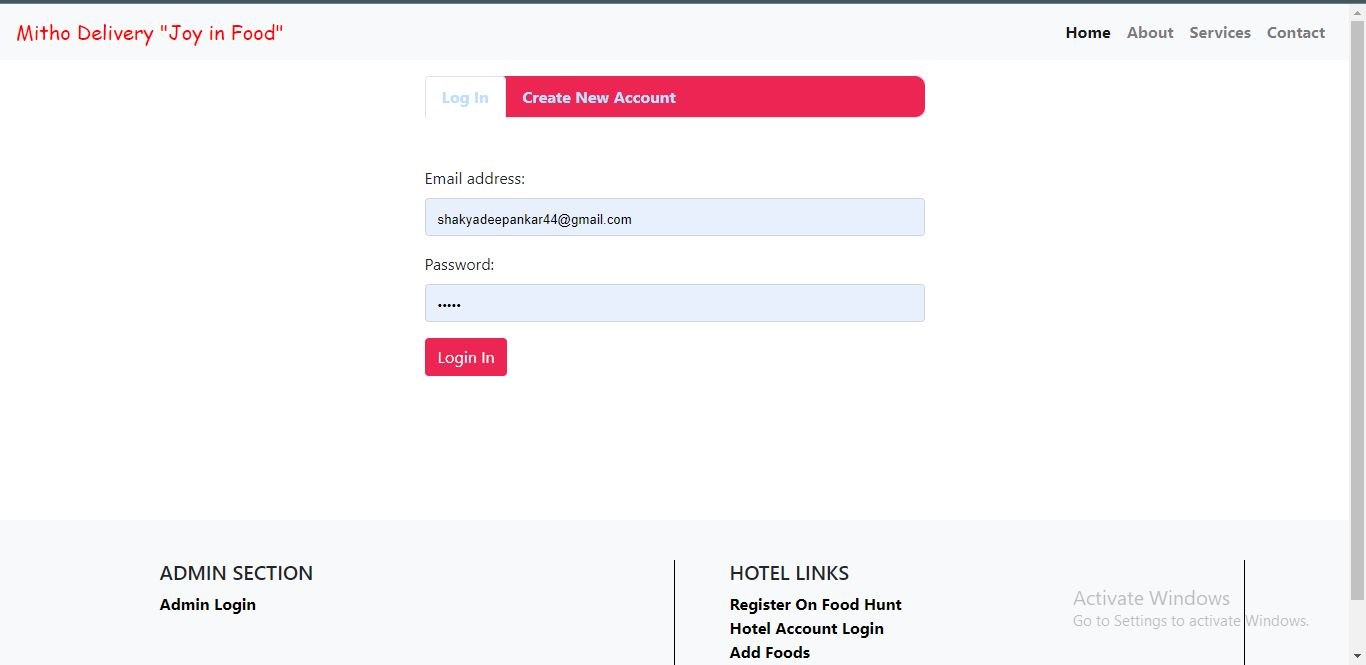
\includegraphics[scale=0.4]{img/Graphics/login ui.JPG}
    \caption{Login Page UI}
\end{figure}

Below is the home page ui of our website.
\begin{figure}[h]
    \centering
    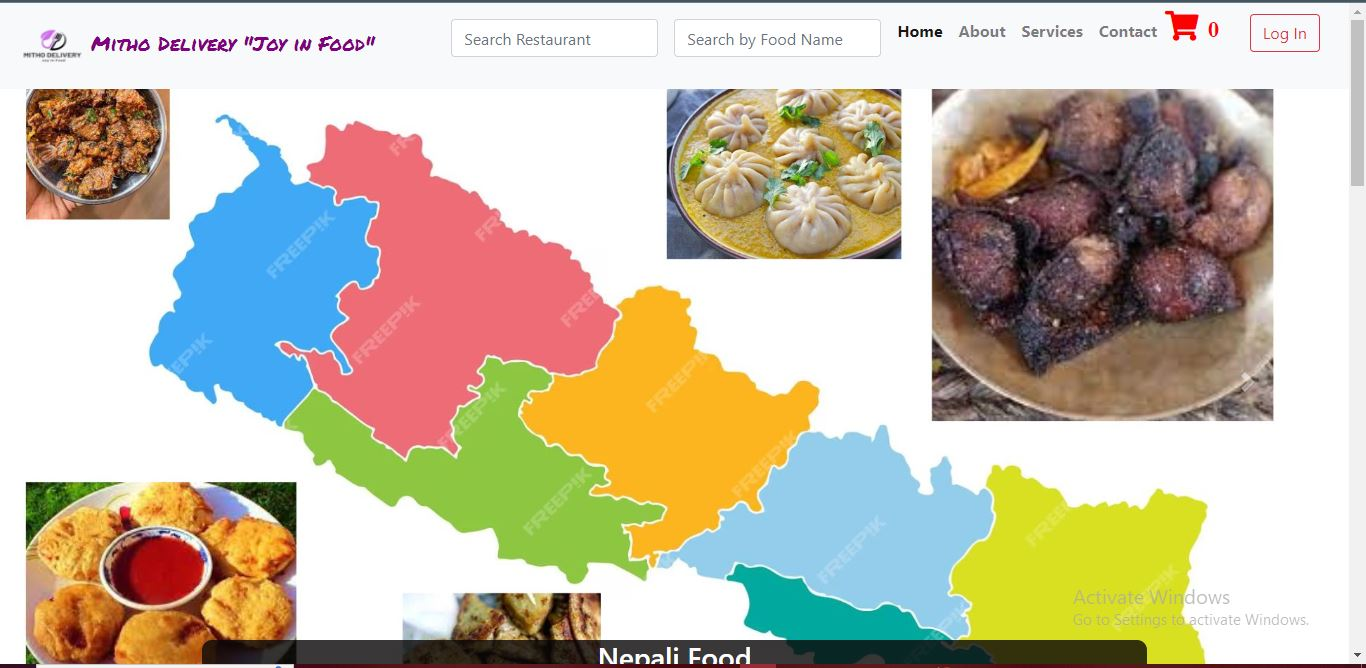
\includegraphics[height=7cm]{img/Graphics/home ui.JPG}
    \caption{Home Page UI}
\end{figure}

\newpage
Below is the cart page of our website.
\begin{figure}[h]
    \centering
    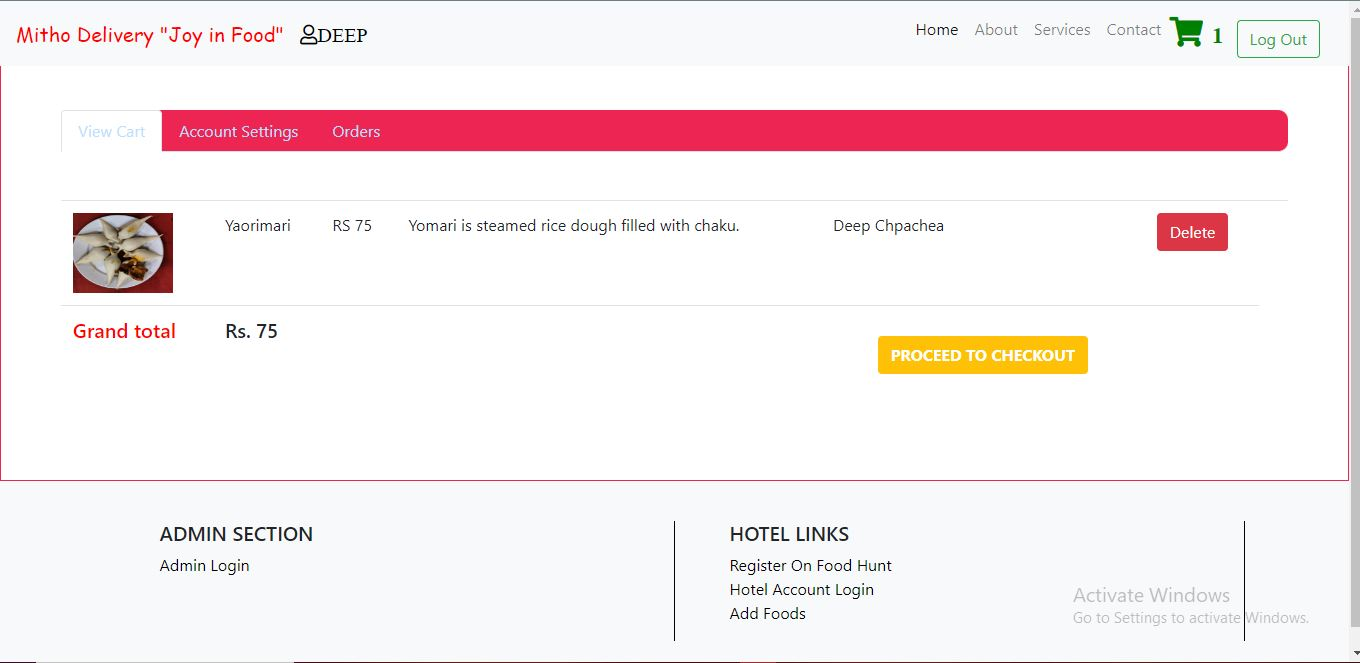
\includegraphics[scale=0.4]{img/Graphics/cart ui.JPG}
    \caption{Cart UI}
\end{figure}

\newpage
\subsection{Architectural Design}
Architectural Design is the process of defining a collection of hardware and software components and their interfaces to establish the framework for the development of a computer system.
\begin{figure}[h]
    \centering
    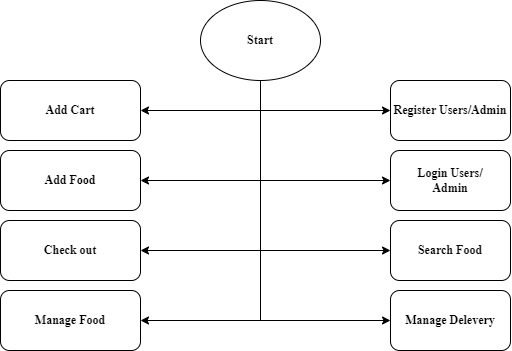
\includegraphics[scale=0.8]{img/Graphics/ARCHETUREDESIGN.png}
    \caption{Architectural Design}
\end{figure}

\newpage
\subsection{Database schema design}
A database schema defines how data is organized within a relational database; this is inclusive of logical constraints such as, table names, fields, data types, and the relationships between these entities. 
\begin{figure}[h]
    \centering
    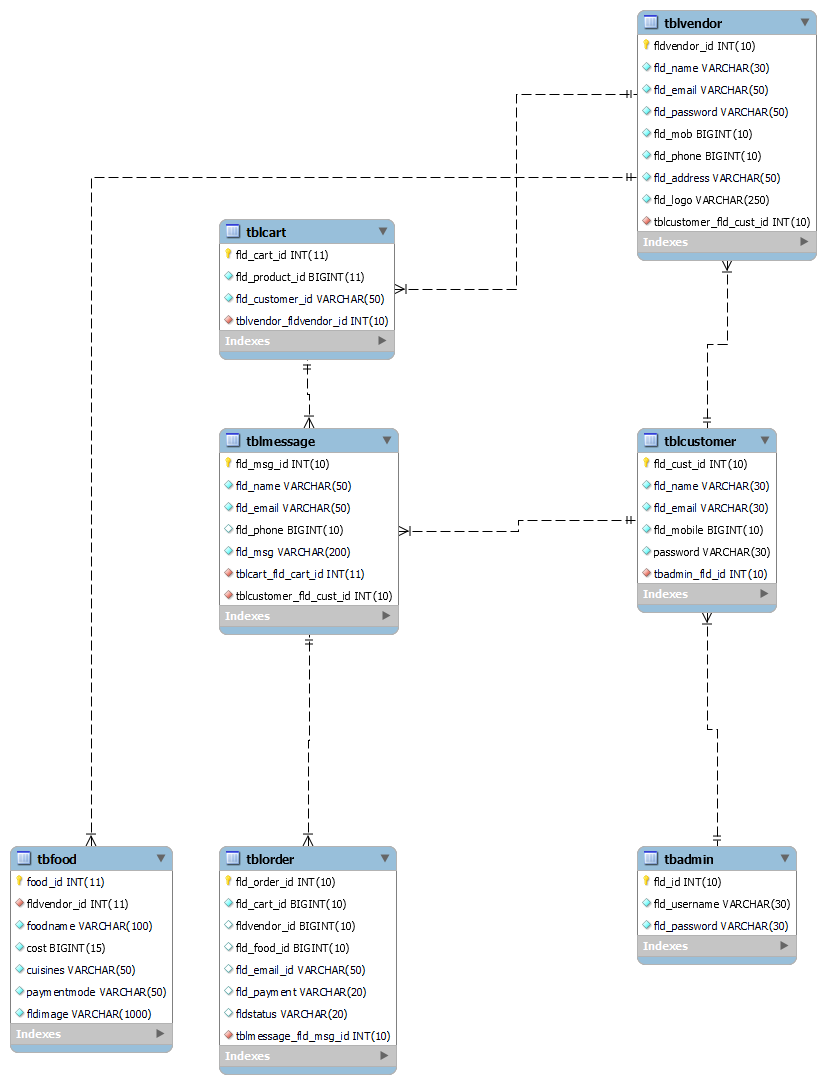
\includegraphics[scale=0.4]{img/Graphics/database.png}
    \caption{Database schema design}
\end{figure}
